\graphicspath{{Chapter1/Figs/}}

\chapter{Joint profiling of chromatin accessibility DNA methylation and transcription in single cells}

\section{Introduction to single-cell (multi-) omics sequencing}

Single-cell profiling techniques have provided an unprecented opportunity to study cellular heterogeneity at multiple molecular levels. The maturation of single-cell RNA-sequencing technologies has enabled the identification of transcriptional profiles associated with lineage diversification and cell fate commitment \cite{Kolodziejczyk2015,Griffiths2018,Papalexi2017,Patel2014}. Yet, the accompanying epigenetic changes and the role of other molecular layers in driving cell fate decisions still remains poorly understood. Consequently, the profiling the epigenome at the single-cell level is receiving increasing attention, but without associated transcriptomic readouts, the conclusions that can be extracted from epigenetic measurements are limited \cite{Stuart2019,Kelsey2017,Griffiths2018}.

\subsection{Single-cell RNA sequencing} \label{section:rna_expresssion}

single-cell RNA sequencing (scRNA-seq) protocols differ extensively in terms of scalability, costs and sensitivity \cite{Svensson2018, Lafzi2018}. Broadly speaking, they can be classified into plate-based and droplet-based methods. In plate-based methods such as CEL-seq \cite{Hashimshony2012} and Smart-seq\cite{Ramskold2012, Picelli2014}, cells are isolated using micropipettes or flow cytometry into individual wells of a plate, where the library preparation is performed. Although plate-based strategies have limitations in terms of throughput and scalability, their main advantage is the higher quality of libraries and the full length transcript information (in the case of Smart-seq) which enables a more accurate quantification of splice variants\cite{Huang2017}, allele-specific fractions\cite{Deng2014} and RNA velocity information \cite{LaManno2018}.
	
Droplet-based methods are based on the use of droplet microfluidics technology \cite{Zhang2019}. By capturing cells in individual droplets, each containing all necessary reagents for library preparation, this protocol allows the profiling of thousands of cells in a single experiment. These class of methods include InDrop \cite{Klein2015,Zilionis2016}, Drop-seq\cite{Macosko2015} and the comercial 10x Genomics Chromium \cite{Zheng2017}. As a trade-off, the increased high throughput of droplet-based approaches comes at the expense of reduced sensitivity\cite{Ziegenhain2017,Wang2019,Svensson2017}.

More recently, a third type of scRNA-seq methodology emerged based on a combinatorial cellular indexing strategy \cite{Cao2017,Rosenberg2018,Cao2019}, which has permitted the sequencing of more than a milion cells in a single experiment for a fraction of the cost of other methods, yet with much lower sensitivity.

\subsection{Single-cell sequencing of the epigenome}

While the large majority of single-cell studies are focused on capturing the mRNA expression, transcriptomic readouts provide a single dimension of cellular heterogeneity and hence contain limited information to characterise the molecular determinants of phenotypic variation \cite{Ritchie2015}. Consequently, gene expression markers have been identified for a myriad of biological systems, but the role of the accompanying epigenetic changes in driving cell fate decisions remains poorly understood \cite{Griffiths2018,Kelsey2017,Bheda2014}.

\subsubsection{DNA methylation} \label{section:dna_methylation}
DNA methylation is a stable epigenetic modification that is strongly associated with transcriptional regulation and lineage diversification in both developmental and adult tissues \cite{Jin2018, Harrison2011, Lee2014, Smith2013}. Its classical roles include the silencing of repeating elements, inactivation of the X chromosome, gene imprinting, and repression of gene expression \cite{Jones2012}. Consistently, the disruption of the DNA methylation machinery is associated with multiple dysfunctions, including cancer \cite{Baylin2011}, autoimmune diseases \cite{Liu2013} and neurological disorders \cite{Amir1999}.\\
In mammalian genomes, DNA methylation predominantly occurs at CpG dinucleotides (mCG). The presence of DNA methylation in non-CpG contexts (mCH) has been confirmed, albeit its functional role remains controversial \cite{He2015, Ramsahoye2000, Lister2009}.

% The establishment of DNA methylation signatures begin during development by the interplay of \textit{de novo} methylation and demethylation events. In mammals, methylation events are orchestrated by three different DNA methyltransferase enzymes with similar structure but different activity patterns: Dnmt1, Dnmt3a, Dnmt3b.
Alongside developments in scRNA-seq technologies, protocols for the profiling of DNA methylation in single cells also emerged from its bulk counterparts (\Cref{fig:methylation_protocols}), most notably bisulfite sequencing (BS-seq) \cite{Smallwood2014,Guo2013,Gravina2016,Farlik2015}. The underlying principle of BS-seq is the treatment of the DNA with sodium bisulfite before DNA sequencing, which converts unmethylated cytosine (C) residues to uracil (and eventually to thymine (T), after PCR amplification), leaving 5-methylcytosine residues intact. The resulting C$\to$T transitions can then be detected by DNA sequencing \cite{Frommer1992,Clark2016,Clark2017}. Nevertheless, the high degree of DNA degradation caused by the purification steps and the bisulfite treatment impaired the use of conventional BS-seq with low starting amounts of DNA. To address this problem, \cite{Smallwood2014} adapted the post-bisulfite adaptor tagging (PBAT) protocol with multiple rounds of 3' random primer amplification (\Cref{fig:scBS}). When the bisulfite treatment is performed before ligation of adaptors, rather than afterwards, loss of adapter-tagged molecules is minimised, unveiling the potential to use scBS-seq from low-input material. In a proof of concept study, \cite{Smallwood2014} applied scBS-seq on ovulated metaphase II oocytes and mouse ESCs, reporting an average coverage of 3.7 million CpG dinucleotides (17.7\%) per cell.

\begin{figure}[H]
	\centering
	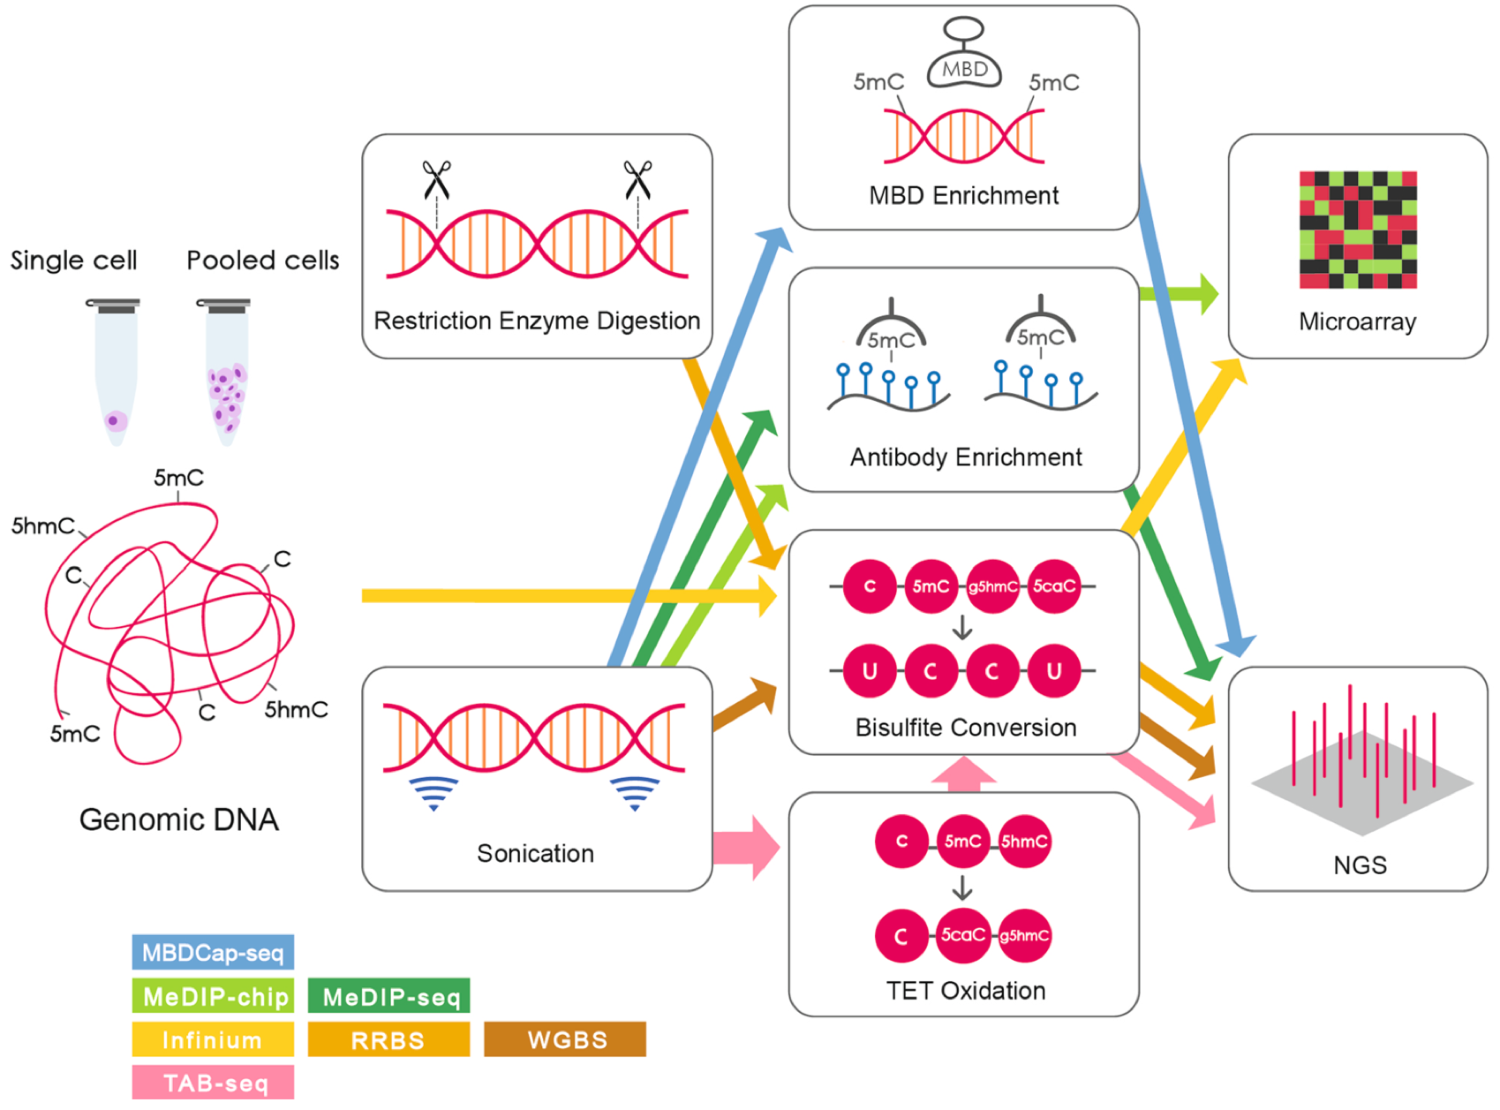
\includegraphics[width=0.8\linewidth]{methylation_protocols}
	\caption[]{Workflow of DNA methylation profiling protocols. Reprinted from \cite{Yong2016}}
	\label{fig:methylation_protocols}
\end{figure}


Alongside scBS, other bulk sequencing methods were also adapted to the single cell resolution, with different trade-offs between coverage and costs. For instance, \cite{Guo2015} adapted the reduced-representation bisulfite sequencing (RRBS-seq) to low starting material by performing all experimental steps before PCR amplification into a single tube. The key principle behind RRBS-seq is to digest the DNA with a restriction endonuclease, followed by a size-selection strategy to enrich for CpG-dense areas \cite{Meissner2005}. This approach significantly reduces sequencing costs at the expense of low coverage in CpG-poor genomic areas, which include repetitive elements, gene bodies and enhancer elements.

\subsubsection{Chromatin accessibility} \label{section:chromatin_accessibility}

In eukaryotes, the genome is packed into a compact complex of DNA, RNA and proteins called chromatin. Several layers of chromatin condensation have been identified, the fundamental unit being the nucleosome, which consists on a string of $\approx$  150bp of DNA wrapped around histone proteins, with linker DNA of $\approx$ 80bp connecting them \cite{Klemm2019,Tsompana2014}. The positioning of the nucleosomes in the nucleus provide an important layer of gene regulation, mostly by exposing or sheltering transcription factors binding sites \cite{Jiang2009}. In general, active regulatory regions tend to have low occupancy of nucleosomes, whereas inactive regions show a high density of nucleosomes \cite{Struhl2013}. Thus, the profiling of DNA accessibility and transcription factor footprints represents an important dimension to understand the regulation of gene expression.

% The N-terminal tails of the histones emerge from the nucleosome and are a strong hotspot for chemical modifications, including methylation, acetylation, phosphorylation and others \cite{Bannister2011}. The complex interaction between a histone modification and the corresponding position, often called the histone code, is an important driver of epigenetic regulation and an active area of research \cite{Zhao2015}.

Traditionally, three main experimental approaches have been used to map chromatin accessibility in a genome-wide and high-throughput manner (\Cref{fig:ChromatinAcc_protocols}): DNase sequencing (DNase-seq) \cite{Song2010}, transposase-accessible chromatin followed by sequencing (ATAC-seq) \cite{Buenrostro2013} and Nucleosome Occupancy and Methylome-sequencing (NOMe-seq) \cite{Kelly2012}. A systematic comparison with a controlled experimental design can be found in \cite{Nordstrom2019}.

\begin{itemize}

	\item \textbf{DNase-seq}: the chromatin is incubated with DNAse I, an enzyme that in low concentrations cuts nucleosome-free regions. Hence accessible sites are released and sequenced \cite{Song2010}. Although this methodology became one of the gold standards to map chromatin accessibility by the ENCODE consortium \cite{ENCODE2012,Thurman2012}, it has now been reported that DNase I introduces significant cleavage biases, thus affecting its reliability to infer transcription factor footprints \cite{He2013}.

	\item \textbf{ATAC-seq}: the chromatin is incubated with hyperactive mutant Tn5 transposase, an enzyme that inserts artifical sequencing adapters into nucleosome-free regions. Subsequently, the adaptors are purified, PCR-amplified  and sequenced. In the recent years it has arguably displaced DNase-seq as the \textit{de facto} method for profiling chromatin accessibility due to its fast and sensitive protocol \cite{Buenrostro2015b,Tsompana2014,Nordstrom2019}.

	\item \textbf{NOMe-seq}: follows a very different strategy than the previous technologies. The idea is to incubate cells with a GpC methyltransferase (M.CviPI), which labels accessible (or nucleosome depleted) GpC sites by DNA methylation. In mammalian genomes, cytosine residues in GpC dinucleotides are methylated at a very low rate \cite{Kilgore2007}. Hence, after M.CviPI treatment followed by bisulfite sequencing, GpC methylation marks can be interpreted as direct read outs for chromatin accessibility. \cite{Kelly2012}. NOMe-seq has a range of appealing properties in comparison with count-based methods such as ATAC-seq or DNAseq-seq. First, one can obtain simultaneous information of CpG DNA methylation with little additional cost, permitting the user to effectively measure two molecular layers for the price of one. Second, the resolution of the method is determined by the frequency of GpC sites within the genome ($\approx$ 1 in 16 bp), rather than the size of a library fragment (usually >100 bp). This allows the quantification of nucleosome positioning and transcription factor footprints at high resolution \cite{Kelly2012,Pott2016,Nordstrom2019}. Third, missing data can be easily discriminated from inaccessible chromatin. This implies that lowly accessible sites will not suffer from increased technical variation (due to low read counts) compared to highly accessible sites.
	The downsides of the approach are the high sequencing depth requirements and the need to discard read outs from GCG positions (21\%) and CGC positions (27\%), as we will discussed later on.	

\end{itemize}


\begin{figure}[H]
	\centering
	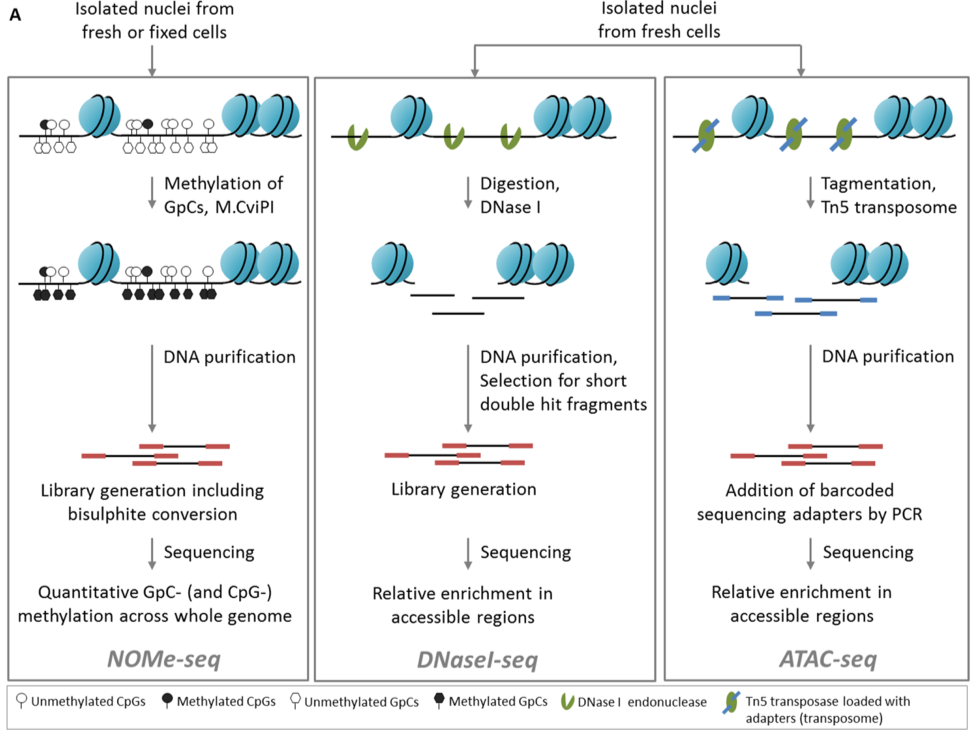
\includegraphics[width=0.8\linewidth]{ChromatinAcc_protocols}
	\caption[]{High-level overview of the workflows for the three main chromatin accessibility assays: NOMe-seq, DNase-seq and ATAC-seq. Reprinted from \cite{Nordstrom2019}. }
	\label{fig:ChromatinAcc_protocols}
\end{figure}

As with DNA methylation, single-cell profiling methods for chromatin accessibility also emerged from its bulk counterparts, including ATAC-seq\cite{Buenrostro2015a}, NOMe-seq \cite{Pott2016} and DNase-seq \cite{Jin2015}. Due to its cost-effective strategy, single-cell ATAC-seq (scATAC-seq) has become the most popular technique to map open chromatin \cite{Cusanovich2015,Cao2018,Chen2018}. Compared to bulk ATAC-seq, scATAC-seq libraries are notably sparse. In a saturated library, \cite{Cusanovich2015} reported a range of $\approx$ 500 to $\approx$ 70,000 mapped reads per cell, with a median of $\approx$ 2500. As the authors report, this represents less than 25\% of the molecular complexity expected from 500-cell bulk experiments. Yet, despite the low coverage, the authors showed that cell-type mixtures can be confidently deconvoluted. Later, in a pioneer effort, \cite{Cusanovich2018b} generated an atlas of chromatin accessibility for different mouse tissues, defining the first \textit{in vivo} landscape of the regulatory genome single-cell resolution.

%- DISCUSS SCALABILITY OF ATAC-SEQ VS NOME-SEQ
% However, the sparse nature of scATAC-seq makes it impractical for the study of heterogeneity in individual regulatory elements. This is addressed mostly by NOMe-seq, which at the expensive of more expensive sequencing and limited scalability, it provides base-pair resolution readouts, even at the single cell resolution \cite{Pott2016}.


\subsection{Multi-modal single-cell sequencing} \label{section:single_cell_multi_modal}

Cellular phenotypes result from the combination of multiple sources of biological information. Undoubtedly, no single "-omics" technology can capture the intricacy of complex molecular mechanisms, but the collective information has the potential to draw a more comprehensive picture of biological processes \cite{Hasin2017,Ritchie2015}. In addition, multi-omics assays have the potential to go beyond snapshots to provide a more dynamic, perhaps even mechanistic, understanding of the connection between molecular layers.


% Motivated by this assumption, multiple omics are being increasingly applied across a wide range of biological domains, including cancer biology \cite{Akavia2010,Gerstung2015}, regulatory genomics \cite{Chen2016}, microbiology \cite{Kim2016} or host-pathogen interactions \cite{Soderholm2016}.

Interestingly, recent technological advances have enabled the profiling of multiple omics in the same single cell. As reviewed in \cite{Stuart2019,Chappell2018}, multi-modal measurements can be obtained using four broad strategies:
\begin{itemize}
	
	\item \textbf{Application of a non-destructive assay before a destructive assay}: a prominent example is the sorting of cells based on protein surface markers using (multiparameter) fluorescence-activated cell sorting (FACS) followed by high-throughput sequencing \cite{Paul2015}. Although simple and efficient, this approach requires prior knowledge of protein surface markers, and is limited by the spectral overlap of fluorescence reporters.

	\item \textbf{Physical isolation of different cellular fractions followed by high-throughput sequencing}: this technique was pioneered with the introduction of genome and transcriptome sequencing (G\&T-seq) \cite{Macaulay2015}. After cell lysis, the mRNA fraction is separated from the genomic DNA fraction using biotinylated or paramagnetic oligo(dT) beads, followed by the independent sequencing of the mRNA and the DNA. This strategy allows the simultaneous profiling of transcriptomic measurements with (epi)-genomic measurements, including DNA sequence, copy number variation, DNA methylation or chromatin accessibility \cite{Macaulay2015,Hou2016,Angermueller2016,Hu2016}.

	\item \textbf{Conversion of different molecular layers to a common format that can be measured using the same readout}: prominent examples are the simultaneous measure of surface proteins and mRNA expression as in Cellular indexing of transcriptomes and epitopes by sequencing (CITE-seq\cite{Stoeckius2017}) and RNA expression and protein sequencing assay (REAP-seq\cite{Peterson2017}). The idea is to incubate cells with antibodies tagged with oligonucleotides that target specific protein surface proteins. This allows both protein surface markers and mRNA levels to be simultaneously measured using a single sequencing round. Notably, this strategy is significantly more powerful than FACS, as the DNA barcodes can be resolved at the sequence level with much higher sensitivity.\\
	A second prominent example is NOMe-seq, described in \Cref{section:chromatin_accessibility}. By labelling accessibile GpC sites with DNA methylation marks, one can simultaneously measure endogenous DNA methylation and chromatin accessibility using a single bisulfite sequencing assay.
\end{itemize}

% - MENTION SNARE-SEQ
% - MENTION SCI-CAR
% - MENTION scNMT-seq here???

Although single-cell multi-modal have proven successful, they still face numerous difficulties, both from the experimental and the computational front, including limited scalability, low coverage and high levels of technical noise. These difficulties, also inherent to single-cell uni-modal techniques, generally get exacerbated when doing multi-modal profiling. Quoting Cole Trapnell: \textit{When you do a multi-omic assay, you are combining all the bad things from multiple protocols}.

% A clear example is scNMT-seq, where an almost \%50 decrease of coverage is observed in DNA methylation with respect to scM\&T-seq. Similarly, chromatin accessible measurements in sci-CAR\cite{Cao2018a} showed \~10-fold less complexity than scATAC-seq.\\
A clear example is sci-CAR \cite{Cao2018a}, a combinatorial indexing strategy that combines scRNA-seq and scATAC-seq to profile gene expression and chromatin accessibility in the same cell. This is a promising approaches that reported, for the first time, the profiling of both modalities in thousands of cells. However, the  chromatin accessibility modality yielded \~10-fold less complexity than (already sparse) scATAC-seq experiments.\\

I envision that a significant effort will be placed in the next years to obtain more scalable and cheaper multi-modal measurements from single cells. However, As cost and scalability remain a barrier for high-resolution multi-modal technologies, the use of computational methods that integrate multi-modal measurements from different sets of cells will be a cornerstone of single-cell analysis.


